\newpage
\chapter{Experimental Results}
\label{experiment_results}
\lhead{\emph{Experimental Results}}
We first present a full replication and extension of the work by
\citet{radDeliberationSinglePeakednessCoherent2021}. Then we present the
simulations based on our model of meta-deliberation, as well as the results of
the sensitivity analysis on both models. All code for the replication, main
experiment and visualizations can be found in
\href{https://github.com/amirsahrani/master_thesis}{this Repository}.


\section{Replication}
We are able to fully replicate the results found by
\citet{radDeliberationSinglePeakednessCoherent2021},  in \Cref{fig:rep_cyclic}
we see that while the bias is less than 0.73, all metric results in a-cyclic
preferences. We also replicate the behavior of the KS metric, where biases in
the range of 0.73-0.85, show even some initial a-cyclic profiles can become
cyclic. \Cref{fig:rep_count} Further explains this by showing that within this
range we always observe 3 unique profile for the KS metric, while DP and CS
have already settled on 6 profiles, thereby representing all possible
preferences. \Cref{fig:rep_condorcet} shows KS introduces ambiguity in the case
that there was a Condorcet winner, resulting in losing the original nice
profile. Finally, the proximity to single-peakedness shows a slightly more
positive note for the KS metric, showing that while the DP and CS bottom out to
the minimum proximity to single-peakedness, KS stays relatively close. Though
this should be taken with a grain of salt, as it is likely a consequence of the
unique preferences being smaller.

\begin{figure}[htbp]
	\centering
	\begin{minipage}{0.45\textwidth}
		\centering
		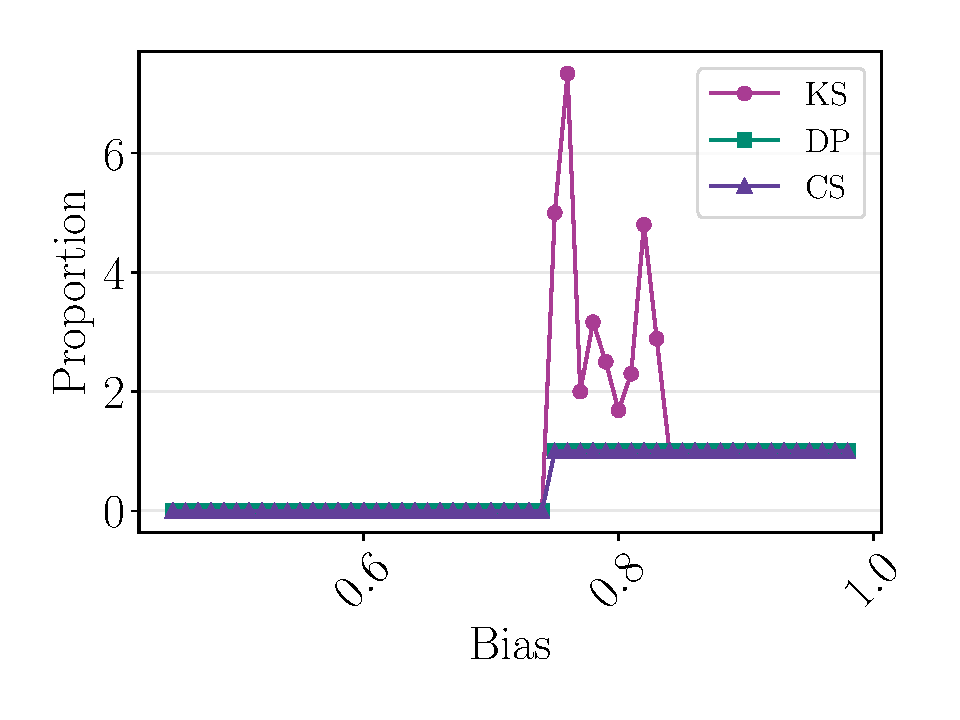
\includegraphics[width=\textwidth]{Figures/cyclic_proportion_Proportion.pdf}
		\caption{The proportion of cyclic profiles remaining, 0 indicating that no cyclic profiles were present after deliberation.}
		\label{fig:rep_cyclic}
	\end{minipage}\hfill
	\begin{minipage}{0.45\textwidth}
		\centering
		\vspace{-9pt}
		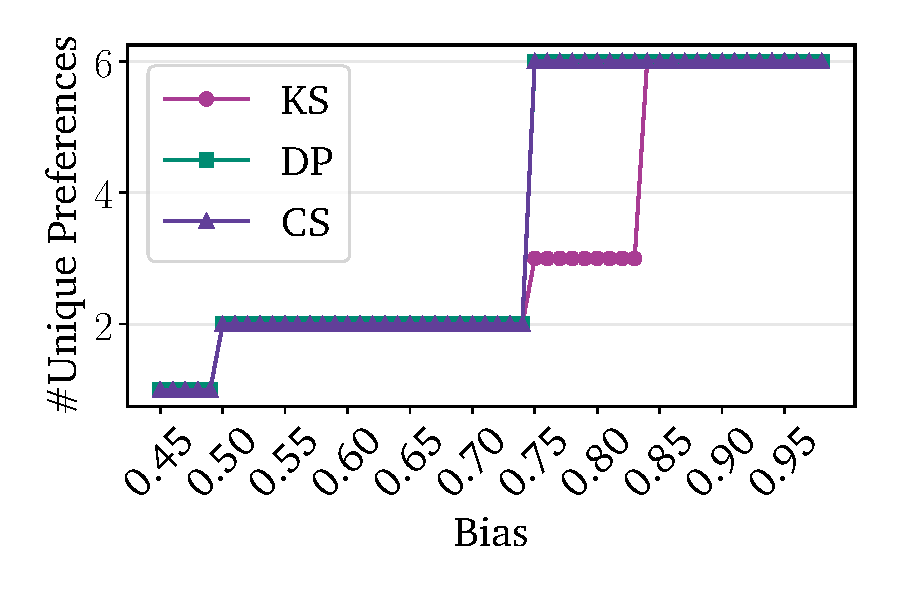
\includegraphics[width=\textwidth]{Figures/unique_Unique Preferences.pdf}
		\caption{Number of unique preferences at the final step of deliberation.}
		\label{fig:rep_count}
	\end{minipage}

	\vspace{1em}

	\begin{minipage}{0.45\textwidth}
		\centering
		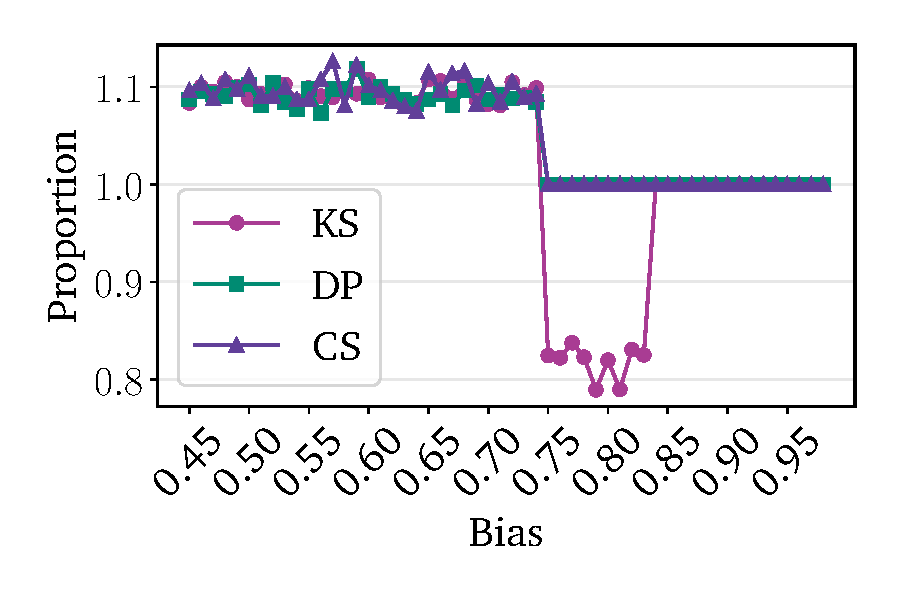
\includegraphics[width=\textwidth]{Figures/condorcet_proportion_Proportion.pdf}
		\caption{The proportion of Condorcet winners left after deliberation, value above one indicate Condorcet winners emerging during deliberation}
		\label{fig:rep_condorcet}
	\end{minipage}\hfill
	\begin{minipage}{0.45\textwidth}
		\centering
		\vspace{-9pt}
		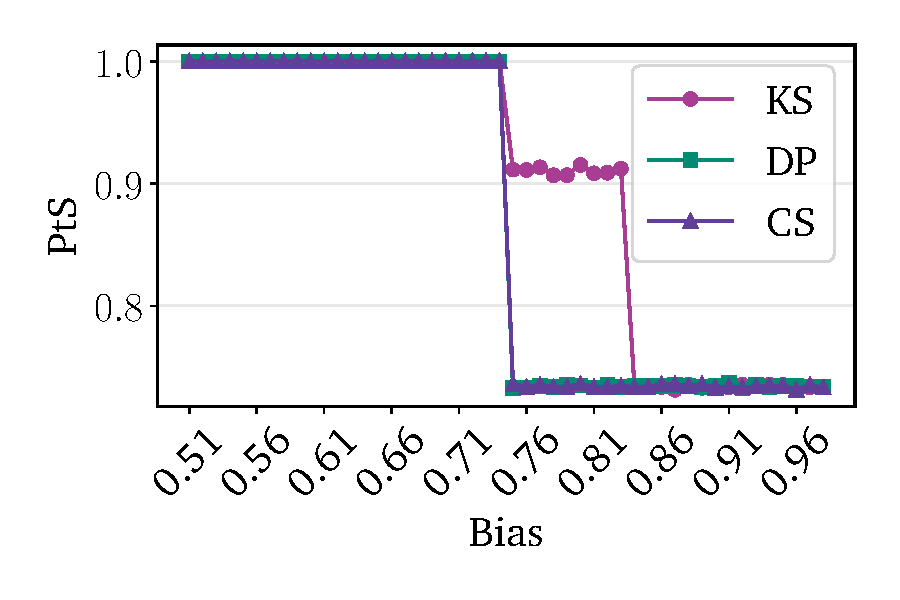
\includegraphics[width=\textwidth]{Figures/sp_proximity_PtS.pdf}
		\caption{Proximity to single-peakedness after deliberation. Proximity to single-peakedness as defined in \Cref{section:related_work}.}
		\label{fig:rep_single_peaked}
	\end{minipage}
\end{figure}

\newpage
\section{DeGroot Model}
\label{degroot_results}

We now present the results of our model based on the DeGroot learning process.
The deliberation group, which is supposed to represent a small group with
deeper talks with everyone on the group, is analysed first. The deliberation
group is modelled as a dense graph, with a few voters. Though the original data
supplied group numbers, for these experiments voters were assigned to their
groups arbitrarily. In terms of the final measures, we focus on whether the
final profiles are cyclic, whether they have a Condorcet winner, home many
unique profiles there are, and their proximity to being singly peaked.
Proximity to single peakedness is measured in two ways. When the simulation
size allows for it, we measure the proximity in terms of the number of voters
that would need to be removed for the full profile to become singly peaked.
This particular method is NP-complete
\cite{erdelyiComputationalAspectsNearly2013}, though it allows for a
2-approximation, we cannot reliably use it for larger groups, given the
sheer number of simulation necessary. The other notion of proximity, which we
will always measure, is the proximity in terms of the number of candidates that
need to be removed for the profile to become singly peaked. This can be done in
$\mathcal{O}(|V| \cdot{} |C| ^3)$\cite{przedmojskiAlgorithmsExperimentsNearly}, though the implementation used is
that of the \texttt{PrefTools} library \cite{preftool}, which implements a slower
$\mathcal{O}(|V| \cdot{} |C|^5)$ algorithm
\cite{erdelyiComputationalAspectsNearly2013}. 



\renewcommand{\arraystretch}{1.2}
\begin{table}
	\centering
	\begin{tabular}{p{4cm}p{0.65\linewidth }}
		\toprule
		Parameter & Description  \\
		\midrule
	\texttt{Number of Voters} & The number of voters in the simulation, representing either the deliberation group, or the control population.\\
	\texttt{Number of Candidates}  & The number of candidates to be voted on. \\
	\texttt{Candidate Generator} & The way the candidates are generated. Either a random voter is selected for each candidate, or 10 random voters get averaged into one candidate.\\
	\texttt{Bias}& The bias all voters have towards their own opinion. \\
	\texttt{Time steps}& The number of deliberation ``steps" the voters undergo.\\
		\bottomrule
	\end{tabular}
	\caption{The parameters of the DeGroot learning based model, as well as their descriptions}
\end{table}

Since the dataset used does not contain full preference rankings, we validate
the explanatory power of the model as follows. We aim to show that under
different numbers of voters and candidates and different ways to generate
candidates, we can find bias factors and deliberation times which minimize the
error of our model. Through showing these positive results for multiple
different (plausible) scenarios we argue that model does capture the learning
process. We then proceed to analyse the results in relation to this dataset,
interpreting the optimal bias values, as well as looking at the rate of
converges given "optimal" parameters. For this analysis, all configurations
were run 100 times. 


\subsection{Optimal parameters}

Between the deliberation group and the control group, if we look at the final
time step, we find that both perform best if the bias is set to be around 1,
though this differs based on the other parameters. This seems to indicate that
for both smaller and larger groups, a voter's opinion is in some sense equally
important as the of  \textit{all} other voters she comes in contact with. In
other words, it does not seem to matter how many people disagree with a voter,
her own opinion holds a constant relative importance.

Looking at the deliberation group, we show the best bias values in the following table:
\begin{table}[ht]
\centering
\begin{tabular}{ccccccc}
\toprule
$n_\text{candidates}$ & $n_\text{voters}$ & MSE (Sample) & MSE (Voter) & Bias (Sample) & Bias (Voter) \\
\midrule
3 & 9  & 0.00747 & 0.00733 & 1.3 & 1.3 \\
3 & 11 & 0.00951 & 0.00969 & 1.2 & 1.0 \\
3 & 13 & 0.00978 & 0.01080 & 1.2 & 1.2 \\
3 & 15 & 0.01409 & 0.01231 & 1.3 & 0.9 \\
5 & 9  & 0.03244 & 0.05191 & 0.8 & 1.1 \\
5 & 11 & 0.05640 & 0.05591 & 1.4 & 0.9 \\
5 & 13 & 0.07609 & 0.08720 & 1.1 & 0.8 \\
5 & 15 & 0.06716 & 0.07476 & 0.9 & 0.9 \\
7 & 9  & 0.07412 & 0.18686 & 1.3 & 1.2 \\
7 & 11 & 0.12538 & 0.17129 & 1.2 & 1.3 \\
\bottomrule
\end{tabular}
\caption{Minimum mean values at time step 151 for each candidate selection method, with corresponding bias.}
\label{tab:min_mean_bias_delib}
\end{table}

Here it is clear that generally the model performs best when both the number of
candidates and the number of voters are low. We also not that though the error
of the different candidate generators are comparable, they in general the
Sample methods seems to results in larger errors, meaning that the model is
less well able to capture circumstances where the alternative's opinions are
not represented in the deliberating population. Finally, we see that The
distribution of best biases skews to values around 1.3, thus indicating that
even while deliberating, people tend to hold their opinion to be \textit{more}
important than that of all other voters.

We investigate this discrepancy between the two candidates generation methods
now, to this end we look at the difference in error for all tested
configuration. 

% Now we T test on everything the Sample and Voter method

\subsection{Convergence}

From \Cref{theory}, we have seen that in the limit some matrices are
convergent, while some are not, in particular if the matrix is aperiodic, this
it is convergent. For the matrices in these simulations, we cannot guarantee 
aperiodicity. Thus, we resort to the following, instead of looking at the
matrices directly, we instead look at the distance between the estimated
support matrix, and the true support matrix, where the distance in the element
wise $\ell_2$ norm. We do the same for the support vectors and the true
opinions.

....


We find ....


\subsection{Single-peaked Preferences}

We now proceed to look at distance to single peaked profiles, look at both
voter removal and candidate removal. We show that for optimal bias, as
deliberation progresses we see an increase in the proximity to single
peakedness.

...
